\section{Vorraussetzungen}
\label{Vorraussetzungen}

%% What you need for building our oscilloscope
%% also reasoning for the devices

\subsection{Geräte}




\subsection{Zusammenspiel}

Alle Geräte zusammen sehen als Schaltplan so aus:
\begin{figure}[h]
	\centering
	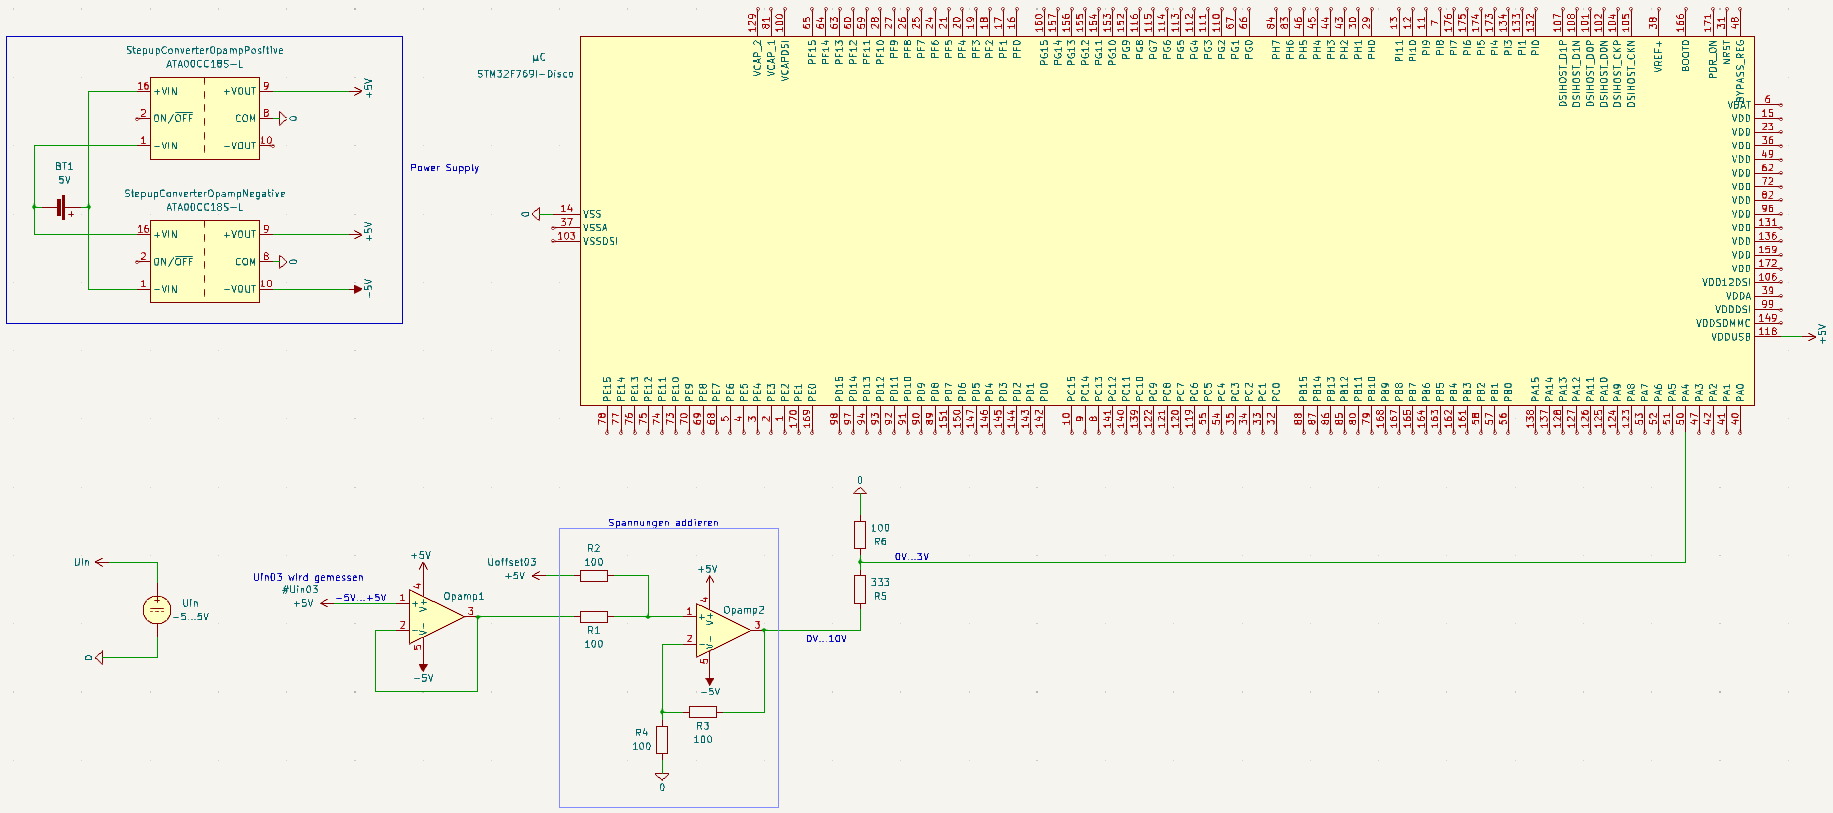
\includegraphics[width=\textwidth, scale=0.5]{images/schematic_opamps2.png}
	\caption{Schematischer Aufbau des Oszilloskops}
\end{figure}


Oszilloskop Eingang ist $U_{in}$ und der Ground $0$. \newline
Für die Messung, muss das Oszilloskop zur gemessenen Spannung parallel geschalten werden,
damit die Spannung am Oszilloskop die gleiche ist, wie die am gemessenen Stromkreis.

\subsubsection{Idee}
Die Eingangsspannung $U_{in}$ liegt im Intervall $[-15, 15] V$,
der GPIO Pin des Mikrocontrollers erlaubt allerdings nur $[0, 3.3] V$. \newline
Folglich muss die Eingangsspannung dahingehend bereinigt werden.
\newline \newline
Hierfür bringen wir die Eingangsspannung erstmal in den positiven Bereich, indem wir
eine Offset Spannung $U_{offset} = 15V$, mithilfe eines Nicht-invertierten Summerverstärkers, erläutert in \ref{Addition einer Offset-Spannung}, dazu addieren. \newline
Der Spannungsbereich ändert sich dadurch zu $[0, 30] V$.
Dieser muss nun lediglich, mithilfe eines Spannungsteilers, siehe \ref{Spannungsteiler}, zu $[0, 3.3] V$ aufgeteilt werden.
Damit der gemessene Stromkreis durch das Oszilloskop nicht belastet wird, muss noch ein Bauteil mit einer hohen Eingangsimpedanz, erläutert in \ref{Unbelastete Eingangsspannung}, vor das ganze Netzwerk geschalten werden.


\subsubsection{Stromversorgung}
Der Mikrocontroller wird über USB mit $5V$ versorgt.
Die beiden Opamps werden durch eine Batterie mithilfe von Stepup Convertern versorgt.

Später werden die einzelnen Schritte ausführlicher erläutert und begründet.



